% $Header: /home/vedranm/bitbucket/beamer/solutions/conference-talks/conference-ornate-20min.en.tex,v 90e850259b8b 2007/01/28 20:48:30 tantau $ %\documentclass[draft]{beamer}
\pdfminorversion=4
\documentclass[]{beamer}
\usepackage{cmacros}
\usepackage{tikz}
\usepackage{cancel}
\usetikzlibrary{shapes.geometric}
\usetikzlibrary{shapes.misc}
\usetikzlibrary{decorations.pathmorphing}
\usetikzlibrary{arrows}
\usetikzlibrary{backgrounds}
\usetikzlibrary{positioning}
\usetikzlibrary{fadings}
\usepackage{units}
\usepackage{listings}
\usepackage{multimedia}
\usepackage{algorithmic}
\usepackage{algorithm}
\usepackage{amssymb}
\tikzset{
  mynodes/.style={text width=1.5cm}
}
\definecolor{dkgreen}{rgb}{0,0.6,0}
\lstset{%
language=Python,
frame=single,
basicstyle=\footnotesize,
keywordstyle=\color{blue},
commentstyle=\color{dkgreen}
}
\definecolor{dkred}{rgb}{0.7,0,0}
\setbeamercolor{alerted text}{fg=dkred}

\newcommand{\eps}{\varepsilon}
\DeclareMathOperator*{\argmax}{arg\,max}
\DeclareMathOperator*{\argmin}{arg\,min}
% This file is a solution template for:

% - Talk at a conference/colloquium.
% - Talk length is about 20min.
% - Style is ornate.

% Copyright 2004 by Till Tantau <tantau@users.sourceforge.net>.
%
% In principle, this file can be redistributed and/or modified under
% the terms of the GNU Public License, version 2.
%
% However, this file is supposed to be a template to be modified
% for your own needs. For this reason, if you use this file as a
% template and not specifically distribute it as part of a another
% package/program, I grant the extra permission to freely copy and
% modify this file as you see fit and even to delete this copyright
% notice. 


\mode<presentation>
{
  \usetheme{default}
  % or ...

  \setbeamercovered{transparent}
  % or whatever (possibly just delete it)

%  \usecolortheme{seahorse}
%  \usecolortheme{rose}
%  \usefonttheme[onlylarge]{structuresmallcapsserif}
%  \usefonttheme[onlysmall]{structurebold}
%  \setbeamerfont{title}{shape=\itshape,family=\rmfamily}
%  \setbeamercolor{title}{fg=red!80!black}
}


\usepackage[english]{babel}
\usepackage[latin1]{inputenc}
\usepackage{times}
\usepackage[T1]{fontenc}

\title{Point spread function reconstruction from the image of a sharp edge}
\author{John Bardsley$^\dagger$, Kevin Joyce$^{\dagger*}$, Aaron Luttman$^{*}$} %, \texttt{kevin1.joyce@umt.edu}}
\date[MUQ '15]{Montana Uncertainty Quantification\\ June 24, 2015}

\institute[The University of Montana] % (optional, but mostly needed)
{
  $^\dagger$The University of Montana\\
  $^{*}$National Security Technologies LLC
}
% - Use the \inst command only if there are several affiliations.
% - Keep it simple, no one is interested in your street address.

%\date[ISPN '80] % (optional, should be abbreviation of conference name)
%{27th International Sumposium of Prime Numbers}
% - Either use conference name or its abbreviation.
% - Not really informative to the audience, more for people (including
%   yourself) who are reading the slides online


% If you have a file called "university-logo-filename.xxx", where xxx
% is a graphic format that can be processed by latex or pdflatex,
% resp., then you can add a logo as follows:

% \pgfdeclareimage[height=0.5cm]{university-logo}{university-logo-filename}
% \logo{\pgfuseimage{university-logo}}



% Delete this, if you do not want the table of contents to pop up at
% the beginning of each subsection:
%\AtBeginSubsection[]
%{
%  \begin{frame}<beamer>{Outline}
%    \tableofcontents[currentsection,currentsubsection]
%  \end{frame}
%}
%

% If you wish to uncover everything in a step-wise fashion, uncomment
% the following command: 

%\beamerdefaultoverlayspecification{<+->}
\begin{document}
\nocite{bardsley2012mcmc,agapiou2014analysis,stuart13bayesian,calvetti2008hypermodels}
\pgfdeclareimage[width=\paperwidth]{titlebackground}{figures/TitleSlide.pdf}
\setbeamertemplate{title page}{
\begin{picture}(0,0)
  \put(-30,-155){%
    \pgfuseimage{titlebackground}
  }
  \put(275,100){\scalebox{.5}{DOE/NV/25946-{}-2491}}
  \put(0,-110.7){%
    \begin{minipage}[b][15em][t]{\textwidth}
      \centering
      \begin{beamercolorbox}[sep=8pt,center]{title}
	\usebeamerfont{title}\inserttitle\par%
%	\ifx\insertsubtitle\@empty%
%	\else%
%	  \vskip0.25em%
%	  {\usebeamerfont{subtitle}\usebeamercolor[fg]{subtitle}\insertsubtitle\par}%
%	\fi%     
      \end{beamercolorbox}%
      \vskip1em\par
      \begin{beamercolorbox}[sep=8pt,center]{author}
	\usebeamerfont{author}\insertauthor
      \end{beamercolorbox}
      \begin{beamercolorbox}[sep=8pt,center]{institute}
	\usebeamerfont{institute}\insertinstitute
      \end{beamercolorbox}
      \begin{beamercolorbox}[sep=8pt,center]{date}
	\usebeamerfont{date}\insertdate
      \end{beamercolorbox}
    \end{minipage}
  }
\end{picture}
}
\setbeamertemplate{navigation symbols}{}

\begin{frame}
  \titlepage
\end{frame}

% Uncomment to add outline of sections
%\begin{frame}{Outline}
%  \tableofcontents[pausesections]
%  % You might wish to add the option [pausesections]
%\end{frame}

% Structuring a talk is a difficult task and the following structure
% may not be suitable. Here are some rules that apply for this
% solution: 

% - Exactly two or three sections (other than the summary).
% - At *most* three subsections per section.
% - Talk about 30s to 2min per frame. So there should be between about
%   15 and 30 frames, all told.

% - A conference audience is likely to know very little of what you
%   are going to talk about. So *simplify*!
% - In a 20min talk, getting the main ideas across is hard
%   enough. Leave out details, even if it means being less precise than
%   you think necessary.
% - If you omit details that are vital to the proof/implementation,
%   just say so once. Everybody will be happy with that.

%% Cygnus pictures
%\begin{frame}
%  \frametitle{Cygnus Radiographic Imaging System}
%  \begin{center}
%  \includegraphics[width=.8\textwidth]{figures/cygnus_pulse_side.pdf}
%  \end{center}
%\end{frame}
%

\section{Modeling Imaging Systems}
\begin{frame}
  \frametitle{Stochastic Imaging Model}
\begin{tikzpicture}[scale=.8,every node/.style={minimum size=1cm},on grid] 
  \def\myxslant{0.1}
  \def\myyslant{-0.4}

    \begin{scope}[
            xshift=50,
            every node/.append style={
            xslant=\myxslant,yslant=\myyslant},xslant=\myxslant,yslant=\myyslant
    ]
	\node[shape = rectangle, anchor=south west, draw] (left) at (0,0){\includegraphics[width=20mm]{figures/roentgen_hand.png}};
    \end{scope}

    \begin{scope}[
	    yshift=-40,
    ] 
%      \node[anchor=south west] (fruit) at (0,0){\includegraphics[width=20mm]{figures/hand.pdf}};
    \end{scope}

    \begin{scope}[
            xshift=180,
            every node/.append style={
            xslant=\myxslant,yslant=\myyslant},xslant=\myxslant,yslant=\myyslant
    ]
	\node[shape = rectangle, anchor=south west, draw] (mid) at (0,0){\includegraphics[width=20mm]{figures/roentgen_hand_blur.pdf}};
    \end{scope}

    \begin{scope}[
            xshift=300,
            every node/.append style={
            xslant=\myxslant,yslant=\myyslant},xslant=\myxslant,yslant=\myyslant
            ]
        %\fill[white,fill opacity=0.6] (0,0) rectangle (5,5);
	\node[anchor=south west] (right) at (0,0){\includegraphics[width=20mm]{figures/roentgen_hand_blur.pdf}};
        \draw[step=1mm, black] (0,0) grid (2.8,2.1); %defining grids
    \end{scope}
    	
%    %putting arrows and labels:
    \node at (2,2.5) (label1) {Ideal Image};
    \draw[-latex,thick] (2,-1.5) to node[below] {Image system response}  (7.5,-1.5);
    \node at (4.65,-3) (math1) {$\displaystyle{\int \alert{k(x-s)}\cdot \,ds }$};

    \node at (12,2.5) (label2) {Measured image};
    \draw[-latex,thick] (9,-1.5) to node[below]{Measurement error} (13.2,-1.5);
    \node at (11,-3) (math1) {$+\vect \eps \sim N(\vect 0,\lambda^{-1} \vect I)$};

    \draw[-latex,thick,bend right] (12,3) to node[below]{Inverse problem}(2,3);
\end{tikzpicture}
\end{frame}

\begin{frame}
  \frametitle{Point Spread Function Estimation}
\begin{tikzpicture}[scale=.8,every node/.style={minimum size=1cm},on grid] 
  \def\myxslant{0.1}
  \def\myyslant{-0.4}

    \begin{scope}[
            yshift=-20,
            every node/.append style={
            xslant=\myxslant,yslant=\myyslant},xslant=\myxslant,yslant=\myyslant
    ]
    \pgfmathsetmacro{\cubex}{1}
    \pgfmathsetmacro{\cubey}{1}
    \pgfmathsetmacro{\cubez}{2}
    \draw[red,thick] (\cubex/2,\cubey/2,0) -- ++(3,3,3);
    \draw[gray,fill=black] (0,0,0) -- ++(-\cubex,0,0) -- ++(0,-\cubey,0) -- ++(\cubex,0,0) -- cycle;
    \draw[gray,fill=black] (0,0,0) -- ++(0,0,-\cubez) -- ++(0,-\cubey,0) -- ++(0,0,\cubez) -- cycle;
    \draw[gray,fill=black] (0,0,0) -- ++(-\cubex,0,0) -- ++(0,0,-\cubez) -- ++(\cubex,0,0) -- cycle;
    \end{scope}

    \begin{scope}[
            xshift=40,
            every node/.append style={
            xslant=\myxslant,yslant=\myyslant},xslant=\myxslant,yslant=\myyslant
    ]
    \draw (0,0) rectangle (2.8,2.2);
    \end{scope}

    \begin{scope}[
            xshift=180,
            every node/.append style={
            xslant=\myxslant,yslant=\myyslant},xslant=\myxslant,yslant=\myyslant
    ]
	\draw (0,0) rectangle (2.8,2.2);
	\tikzfading[name=fade out,inner color = transparent!0,outer color = transparent!100]
	\draw[path fading=fade out, fill=red,red] (1,1.2) circle (.1);
    \end{scope}

    \begin{scope}[
            xshift=300,
            every node/.append style={
            xslant=\myxslant,yslant=\myyslant},xslant=\myxslant,yslant=\myyslant
            ]
        %\fill[white,fill opacity=0.6] (0,0) rectangle (5,5);
	\draw[path fading=fade out, fill=red,red] (1,1.2) circle (.1);
        \draw[step=1mm, black] (0,0) grid (2.8,2.2); %defining grids
    \end{scope}
    	

%    %putting arrows and labels:
    \node at (2,2.5) (label1) {Point Source};
    \draw[-latex,thick] (2,-1.5) to node[below] {Image System Response} (7.5,-1.5);
    \node at (4.65,-3) (math1) {$\displaystyle{\int \alert{k(x-s)} \delta(s)\,ds = \alert{k(x)}}$};

    \node at (7,2.5) (label3) {Impulse Response};

    \node at (12,2.5) (label2) {PSF estimate};
    \draw[-latex,thick] (9,-1.5) to node[below]{Measurement error} (13.2,-1.5);
    \node at (11,-3) (math1) {$+\vect \eps \sim N(\vect 0,\lambda^{-1} \vect I)$};

\end{tikzpicture}
\end{frame}

\begin{frame}
  \frametitle{Point Spread Function Estimation}
\begin{tikzpicture}[scale=.8,every node/.style={minimum size=1cm},on grid] 
  \def\myxslant{0.1}
  \def\myyslant{-0.4}

    \begin{scope}[
            xshift=40,
            every node/.append style={
            xslant=\myxslant,yslant=\myyslant},xslant=\myxslant,yslant=\myyslant
    ]
    \draw (0,0) rectangle (2.8,2.2);
    \draw[fill=black] (0,0) rectangle (1,2.2);
    \end{scope}

    \begin{scope}[
            yshift=-20,
            every node/.append style={
            xslant=\myxslant,yslant=\myyslant},xslant=\myxslant,yslant=\myyslant
    ]
    \draw[x=.314cm,y=.2cm,z=.2cm,thick,-latex,red] (0,0,0) 
      sin ++(0,1,1) cos ++(0,-1,1) sin ++(0,-1,1) cos ++(0,1,1) 
      sin ++(0,1,1) cos ++(0,-1,1) sin ++(0,-1,1) cos ++(0,1,1)
      sin ++(0,1,1) cos ++(0,-1,1) sin ++(0,-1,1) cos ++(0,1,1);
    \draw[x=.314cm,y=.2cm,z=.2cm,thick,-latex,red] (-2,0,0) 
      sin ++(0,1,1) cos ++(0,-1,1) sin ++(0,-1,1) cos ++(0,1,1) 
      sin ++(0,1,1) cos ++(0,-1,1) sin ++(0,-1,1) cos ++(0,1,1) 
      sin ++(0,1,1) cos ++(0,-1,1) sin ++(0,-1,1) cos ++(0,1,1);
    \draw[x=.314cm,y=.2cm,z=.2cm,thick,-latex,red] (-4,0,0) 
      sin ++(0,1,1) cos ++(0,-1,1) sin ++(0,-1,1) cos ++(0,1,1) 
      sin ++(0,1,1) cos ++(0,-1,1) sin ++(0,-1,1) cos ++(0,1,1) 
      sin ++(0,1,1) cos ++(0,-1,1) sin ++(0,-1,1) cos ++(0,1,1);

    \pgfmathsetmacro{\cubex}{2}
    \pgfmathsetmacro{\cubey}{2.5}
    \pgfmathsetmacro{\cubez}{1}
    \draw[black,fill=gray,opacity=.75] (3.7,3,0) -- ++(-\cubex,0,0) -- ++(0,-\cubey,0) -- ++(\cubex,0,0) -- cycle;
    \draw[black,fill=gray,opacity=.75] (3.7,3,0) -- ++(0,0,-\cubez) -- ++(0,-\cubey,0) -- ++(0,0,\cubez) -- cycle;
    \draw[black,fill=gray,opacity=.75] (3.7,3,0) -- ++(-\cubex,0,0) -- ++(0,0,-\cubez) -- ++(\cubex,0,0) -- cycle;

    \draw[x=.314cm,y=.2cm,z=.2cm,thick,-latex,red] (4,0,0) 
      sin ++(0,1,1) cos ++(0,-1,1) sin ++(0,-1,1) cos ++(0,1,1) 
      sin ++(0,1,1) cos ++(0,-1,1) sin ++(0,-1,1) cos ++(0,1,1);
    \draw[x=.314cm,y=.2cm,z=.2cm,thick,-latex,red] (2,0,0) 
      sin ++(0,1,1) cos ++(0,-1,1) sin ++(0,-1,1) cos ++(0,1,1) 
      sin ++(0,1,1) cos ++(0,-1,1) sin ++(0,-1,1) cos ++(0,1,1);
    \end{scope}

    \begin{scope}[
            xshift=180,
            every node/.append style={
            xslant=\myxslant,yslant=\myyslant},xslant=\myxslant,yslant=\myyslant
    ]
	\draw (0,0) rectangle (2.8,2.2);
	\tikzfading[name=fade left,left color = transparent!0,right color = transparent!100]
	\draw[path fading=fade left,fading transform={rotate=-30},fill=black] (.9,0) rectangle (1,2.2);
	\draw[fill=black] (0,0) rectangle (.9,2.2);
    \end{scope}

    \begin{scope}[
            xshift=300,
            every node/.append style={
            xslant=\myxslant,yslant=\myyslant},xslant=\myxslant,yslant=\myyslant
            ]
	\draw (0,0) rectangle (2.8,2.2);
	\tikzfading[name=fade left,left color = transparent!0,right color = transparent!100]
	\draw[path fading=fade left,fading transform={rotate=-30},fill=black] (.9,0) rectangle (1,2.2);
	\draw[fill=black] (0,0) rectangle (.9,2.2);
        \draw[step=1mm, black] (0,0) grid (2.8,2.2); %defining grids
    \end{scope}
    	

%    %putting arrows and labels:
    \node at (2,2.5) (label1) {Heaviside function};
    \draw[-latex,thick] (2,-1.5) to node[below] {Image System Response} (7.5,-1.5);
    \node at (4.65,-3) (math1) {$\displaystyle{f(x)=\int \alert{k(x-s)} E(s)\,ds}$};

    \node at (7,2.5) (label3) {Edge Spread};

    \node at (12,2.5) (label2) {Noisey Data};
    \draw[-latex,thick] (9,-1.5) to node[below]{Measurement error} (13.2,-1.5);
    \node at (11,-3) (math1) {$+\vect \eps \sim N(\vect 0,\lambda^{-1} \vect I)$};

\end{tikzpicture}
\end{frame}

%\begin{frame}
%  \frametitle{Cygnus Radiographic Imaging System}
%  \begin{center}
%  \includegraphics[width=.5\textwidth]{figures/cygnus_pictures.pdf}
%
%  [\emph{Cygnus Performance in Subcritical Experiments}, J. Smith et.al.]
%  \end{center}
%\end{frame}


\begin{frame}[t]
  \frametitle{Underdetermined Inverse problem}
  \vspace{-1em}
  \begin{align*}
    \color{blue}{f(x_i)} &= \int_{-\infty}^\infty\int_{-\infty}^\infty \alert{k(s,t)}E(x_i-s)dtds + \eps_i
  \end{align*}
  \hspace{-2em}
    %\begin{tikzpicture}[show background grid,pic/.style={inner sep=0pt,above right}]
    \begin{tikzpicture}[pic/.style={inner sep=0pt,above right}]
      %\fill (0,0) circle (2pt);


      \node[pic] at (-1,2) (conv1)     { \includegraphics[width=.5\textwidth]{figures/2d_radial_convolution_blank1.pdf} };
      \node[pic] at (5,2.5) (conv2)    { \includegraphics[width=.5\textwidth]{figures/2d_radial_convolution_blank2.pdf} };
      \node[pic] at (5.2,0) (lineout)  { \includegraphics[width=.5\textwidth]{figures/typical_line_out.pdf} };

      \tikzfading[name=fade out,inner color = transparent!0,outer color = transparent!80]
      \draw[fill=red,path fading=fade out] (2.1,1.2) circle (1);


      \node at (0,4) (t) {\footnotesize $t$};
      \node at (1.4,3) (s) {\footnotesize $s$};
      \node at (1.6,6) (y) {\footnotesize $y$};

      \path[bend left,dotted,-latex] (5.7,.8) edge node[above]{??} (3.2,.8);
      \path[bend left,-latex] (3.2,5.8) edge node[above]{\footnotesize System Response} (6,5.8);

    \end{tikzpicture}
\end{frame}

\begin{frame}[t]
  \frametitle{Radially Symmetric PSF}
  \vspace{-.5em}
  {\footnotesize
  If we assume radial symmetry, \alert{$k(x,y) = \rho(\sqrt{x^2+y^2})$}, and that the edge is indicated at $x=0$ by $E$, then
  \begin{align*}
    f(x_i) 
     &= \int_{-\infty}^\infty\int_{-\infty}^\infty k(s,t)E(x_i-s)dtds + \eps_i\\
     &= \int_0^\infty\rho(r) \left(\int_0^{2\pi} E(x_i - r\cos \theta)d \theta \right)\,r dr + \eps_i\\
     &= \int_0^\infty\rho(r) \cdot g(x_i,r)\,r dr + \eps_i.
  \end{align*}

  \begin{center}
\begin{tikzpicture}[scale=.8]
  \draw (0,-2.2) -- (0,2.2);
  \draw (-3,0) -- (3,0);
  \draw[dotted] (-2.5,-2.2) node[below]{\footnotesize$x<-r$} -- (-2.5,2.2);
  \draw[dotted] (2.5,-2.2) node[below]{\footnotesize$x>r$} -- (2.5,2.2);
  \draw[dotted] (-1,-2.2) node[below right]{\footnotesize$|x|\le r$} -- (-1,2.2);

  \draw (0,0) circle[radius=2];
  \draw[very thick,red,domain=120:240] plot ({2*cos(\x)},{2*sin(\x)});
  \draw (0,0) -- (-1,{sqrt(3)});
  \draw (.3,0) node[above right]{$\theta$} arc [radius=.3,start angle=0,end angle=120];
\end{tikzpicture}
  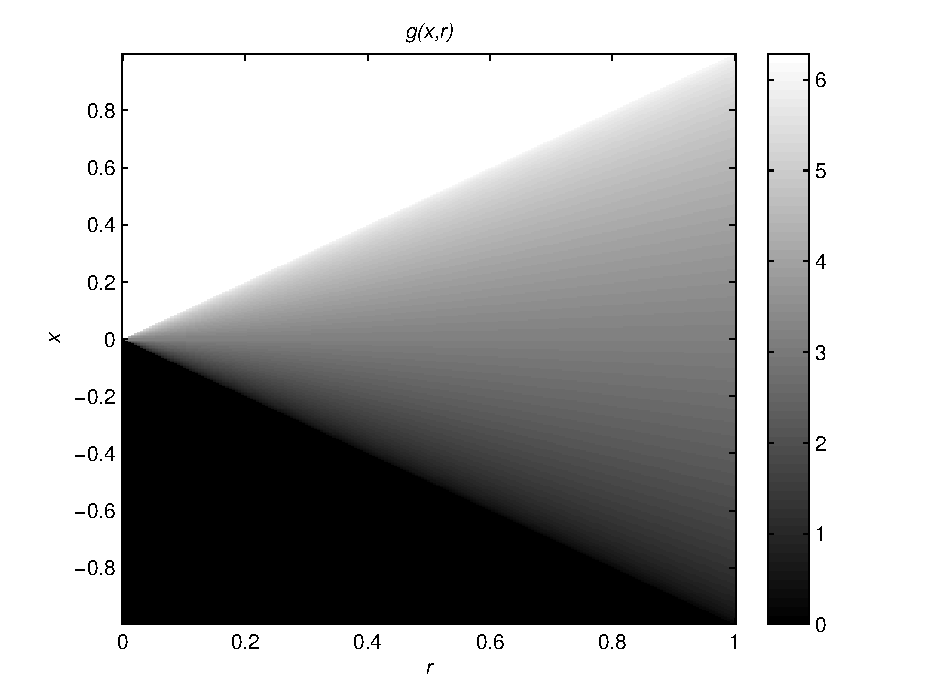
\includegraphics[width=.5\textwidth]{figures/g_function.pdf}

  Observe that $g$ is symmetric about the $x=0$.
  \end{center}
  }
\end{frame}

%\begin{frame}[t]
%  \frametitle{Fredholm Equation of the First Kind and Ill-posedness}
%  Since $g$ is continuous, the integral equation
%  \begin{align*}
%    f(x_i) &= \int_0^\infty\rho(r) \cdot g(x_i,r)\,r dr \\
%    \vect f &= \mathcal G \rho
%  \end{align*}
%  is a \alert{Fredholm integral equation of the first kind}. 
%  {\small
%  \begin{itemize}
%    \itemsep 1em
%    \item The integral operator $\mathcal G$ is \alert{compact}, hence the inverse problem of recovering $\rho$ from $f$ is unstable or \alert{ill-posed}. 
%    \item The integral kernel \alert{$g(x,r)$ is not differentiable for $|x|=r$}, hence discretization of $\mathcal G$ can only guarantee first order convergence.  
%    \item Although ill-posed, the problem is similar to calculating a \alert{regularized derivative} -- which, when cast as an inverse problem, has eigenvalues that converge ``slowly'' to zero and care must be taken for regularization.
%  \end{itemize} 
%  }
%\end{frame}
%
\begin{frame}
  \frametitle{Bayesian Stochastic Inverse Problem}
  {\footnotesize For the inverse problem}
  \begin{equation*}
    \vect f = \mathcal G \rho + \vect \epsilon,
  \end{equation*}
  {\footnotesize
  regularization and uncertainty quantification can be achieved by modeling the PSF as a random quantity with an appropriate prior.
  \begin{itemize}
    \itemsep 1.2em
    \item Measurement error is given by \alert{Gaussian likelihood} with \alert{$\mathrm E\,\vect f = \mathcal G \rho$} and \alert{$\mathrm{Var}\,\vect f = \lambda^{-1}\vect I$}. 
    \item We use a \alert{Gaussian prior} defined implicitly on $k(s,t)$. Denote $\Delta^2_0$ as the squared Laplacian defined on a certain subspace of $L^2(\RR^2)$, then the prior density satisfies \alert{$\mathrm E\, \Delta^2_0 k = 0$} and \alert{$\mathrm{Var}\,\Delta^2_0 k = \delta^{-1} I$} \cite{stuart13bayesian}.
    \item For the polar coordinate map $T(r,\theta)$, the radial symmetry assumption gives $\displaystyle{(\mathcal L\rho)(r) := (\Delta^2_0 k \circ T)(r) = \alert{\left(\frac{1}{r} \frac{d}{dr} r\frac{d}{dr}\right)^2 \rho(r)}}$. Here, we impose a left zero derivative and right zero boundary condition on \alert{$\rho$}.
  \end{itemize}
  }
\end{frame}

\begin{frame}[t]
  \frametitle{Monte Carlo Sampling of the Posterior}
  {\footnotesize
  \begin{itemize}
    \itemsep 1.2em
    \item Since both densities are Gaussian, Bayes Theorem leads to a \alert{posterior density} satisfying 
      $$
	p(\rho|\vect f,\lambda,\delta ) \propto \exp\left( -\frac\lambda2 \|\vect f - \mathcal G\rho\|^2 - \frac\delta2 \| \mathcal L\rho \|^2 \right).
      $$
    \item We impose uninformative Gamma hyper-priors for $\lambda$ and $\delta$ with hyper-parameters $\alpha = 1$ and $\beta = 10^6$ \cite{calvetti2008hypermodels}.%, so that the joint-posterior density satisfies
    \item It can be shown theoretically that for medium to large scale discretizations of the unknown $\rho$, the \alert{Hierarchical Gibbs sampler} gives unsatisfactory samples of $\delta$ as the discretization for $\rho$ becomes more refined \cite{agapiou2014analysis}.
    \item To illustrate this, we implement the hierarchical Gibbs sampler for the discretization $\vect \rho$ at various levels of refinement on a synthetic example. 
  \end{itemize}
  }
\end{frame}

\begin{frame}[t]
  \frametitle{A Synthetic Example}
  A radially symmetric two-dimensional \alert{Gaussian PSF} has the form
  \begin{equation*}
    \rho(r_j) = (2\pi\sigma^2)^{-1} e^{\frac{-r_j^2}{2\sigma^2}} 
  \end{equation*}
  and it can be shown analytically that the analytic forward blur is an \alert{error function}
  \begin{equation*}
    [\mathcal G \rho] (x_i) = \frac 1{\sqrt{2\pi}\sigma} \int_{-\infty}^{x_i} e^{-\frac{s^2}{2\sigma^2}}\,ds
  \end{equation*} 
  \begin{tikzpicture}[pic/.style={inner sep=0pt,above right}]
    \node[pic] at (-1,2.5) (left)     { \includegraphics[width=.4\textwidth]{figures/radial_gaussian_psf.pdf} };
    \node[pic] at (5,2.5) (right)     { \includegraphics[width=.4\textwidth]{figures/radial_gaussian_edgeblur.pdf} };
    \path[bend left,-latex] (3,6) edge node[above]{$\mathcal G$} (6,6); 
  \end{tikzpicture}
\end{frame}

\begin{frame}[t]
  \frametitle{Hierarchical Gibbs Sampler}
  {\footnotesize
  For $\vect \rho$ discretized with $n$ points and $\vect f$ with $2n$ points, the joint posterior density of the unknown and hyperpriors satisfies
  $$
    p(\vect \rho,\lambda,\delta |\vect f) \propto \left(-\frac 12 \Big \langle \vect R (\vect \rho - \vect \mu) , (\vect \rho - \vect \mu)\Big\rangle -\beta(\lambda+\delta)\right),
  $$
  where $\vect R = (\lambda \vect G^* \vect G + \delta \vect L^* \vect L)\vect \rho$ and $\vect \mu = \lambda \vect R^{-1}\vect G^* \vect f$.
  In order to draw efficiently from the conditional density for $\vect \rho$, we use the Cholesky decomposition of $\vect R = \vect S^* \vect S$ which dominates the computation at $O(n^3)$.

  The \alert{Hierarchical Gibbs sample} is: 
  \begin{center}
  \begin{algorithmic}[1]
    \STATE Let $\delta_0$ and $\lambda_0$ be given and set $k=0$.
    \STATE Compute $\vect {R_k} = \vect{S_k}^T \vect{S_k}$. 
    \STATE Draw $\vect \rho_k$ from $N\Big( \lambda_k \vect{R_k}^{-1}\vect G^T\vect f, \vect{R_k}^{-1} \Big)$.
    \STATE Draw $\lambda_{k+1}$ from $\Gamma \Big(n+\alpha,\,\frac12\|\vect{G\rho}_k - \vect f\|^2 - \beta \Big)$
    \alert{\STATE Draw $\delta_{k+1}$ from $\Gamma \Big(n/2+\alpha,\,\frac12\|\vect{L\rho}_k\|^2 - \beta \Big)$}
    \STATE Set $k=k+1$ and return to 2.
  \end{algorithmic}
  \end{center}
  }
\end{frame}

\begin{frame}[t]
  \frametitle{Correlated $\delta$ chains}
  \vspace{-1.2em}
  \begin{center}
    \includegraphics[width=.5\textwidth]{figures/psf_hierarchical_autocor_50.pdf}  \includegraphics[width=.5\textwidth]{figures/psf_hierarchical_chains_50.pdf}\\
    \includegraphics[width=.5\textwidth]{figures/psf_hierarchical_autocor_100.pdf} \includegraphics[width=.5\textwidth]{figures/psf_hierarchical_chains_100.pdf}\\
    \includegraphics[width=.5\textwidth]{figures/psf_hierarchical_autocor_200.pdf} \includegraphics[width=.5\textwidth]{figures/psf_hierarchical_chains_200.pdf}\\
  \end{center}
\end{frame}
\begin{frame}[t]
  \frametitle{Correlated $\delta$ chains}
  \begin{center}
    \includegraphics[width=.5\textwidth]{figures/psf_hierarchical_autocor_500.pdf} \includegraphics[width=.5\textwidth]{figures/psf_hierarchical_chains_500.pdf}\\ 
    \includegraphics[width=.5\textwidth]{figures/psf_hierarchical_autocor_1000.pdf} \includegraphics[width=.5\textwidth]{figures/psf_hierarchical_chains_1000.pdf}\\ 
  \end{center}
\end{frame}

\begin{frame}[t]
\frametitle{Marginalized Posterior Density}
{\footnotesize
In order to marginalize out $\vect \rho$, we \alert{complete the square} of the quadratic form in $\vect \rho$ and integrate out the multivariate Gaussian,
  \begin{align*}
    \int p(\vect \rho,\lambda,\delta|\vect f) d\vect \rho
    &\propto \int (\lambda^2\delta)^{n/2+\alpha} \exp\left(-\frac{\lambda}{2}\|\vect{G\rho} - \vect f\|^2 - \frac{\delta}{2}\|\vect L \vect \rho\|^2 - \beta(\lambda - \delta) \right)d\vect \rho \\
    &= \int(\lambda^2\delta)^{n/2+\alpha}  \exp\left( - \frac 12\Big\langle\vect R(\vect \rho-\vect \mu),(\vect \rho - \vect \mu)\Big\rangle \right.\\
    &\left. \hspace{12em} -\alert{\frac 12U(\lambda,\delta,\vect b)}  -\beta(\lambda - \delta) \right)d\vect \rho\\
    &= (\lambda^2\delta)^{n/2+\alpha}  \alert{ c(\lambda,\delta,\vect f) } \exp\left( -\alert{\frac 12U(\lambda,\delta,\vect b)}  -\beta(\lambda - \delta) \right),
  \end{align*}
  where \alert{$U = \Big\langle (\lambda \vect I - \lambda^2 \vect G\vect R^{-1}\vect G^*)\vect f,\vect f\Big\rangle$} and \alert{$c = \det \vect R ^{-1/2}$}.
\begin{itemize}
  \item To draw from this density, we embed a \alert{Metropolis-Hastings} algorithm within the Gibbs sampler.
  \item Both \alert{$U$} and \alert{$c$} can be carried out using a Cholesky factorization ($O(n^3)$), and will be required for each Metropolis step. 
\end{itemize}
}
\end{frame}

\begin{frame}[t]
  \frametitle{Metropolis-Hastings within Gibbs Sampling}
  \vspace{-1em}
  {\scriptsize
  \begin{itemize}
    \itemsep 1.1em
    \item Since $\delta$ is the problematic parameter, we implment the Metropolis-Hastings step on its conditional marginalized density $p(\delta|\vect f,\lambda)$. 
    \item We use a Gaussian proposal with adaptive variance.  We use an initial variance estimate and support by running a Hierarchical Gibbs sampler.
    \item Due to numerical overflow issues, all computations are carried out on the log scale.
  \end{itemize}
  \begin{algorithmic}[1]
  \STATE Let $\lambda_0$, $\delta_0$ and $\gamma$ be given.
  \STATE Compute $\vect {R_k} = \vect{S_k}^T \vect{S_k}$. 
  \STATE Draw $\vect x_k$ from $N\Big( \vect R_k^{-1}\lambda_k \vect A^T\vect b, \vect R_k^{-1} \Big)$.
  %STATE   \item Draw $\vect z_k$ from  $N(0,\vect I)$, and compute $\vect x_k = \vect S_k^{-1}(\vect z_k + \vect {S_k^T}^{-1}\lambda_k \vect A^T \vect b)$.
  \STATE Draw $\lambda_{k+1}$ from $\Gamma \Big(n/2+\alpha,\,\frac12\|\vect{Ax_k} - \vect b\|^2 - \beta \Big)$.
  \alert{\STATE Set $j = 1$, $\tilde \delta_0 = \frac 1k \sum_{i=1}^k \delta_i$.  Compute $c_0 = \log c(\lambda_k,\tilde \delta_0)$ and then $U_0 = \log U(\lambda_k,\tilde \delta_0,\vect b)$, and $p_0 = \log p(\tilde \delta_0|\vect f \lambda _k)$.
  \WHILE{$j<\tilde M$} 
    \STATE Draw $\tilde \delta_j$ from $N(\tilde \delta_{j-1}, \gamma)$.
    \STATE Compute $U_j = U(\lambda_k,\tilde \delta_j)$, $c_j = c(\lambda_k,\tilde \delta_j)$, and then $p_j = \log p(\tilde \delta_j|\vect f \lambda _k)$.
    \STATE Draw $u_j$ from $\mathrm{Unif}[0,1]$ and if $ p_j - p_{j-1} < \log u_j$ set $p_j = p_{j-1}$ and $\delta_{k} = \tilde \delta_j$. Otherwise, continue.
    \STATE Set $j=j+1$.
  \ENDWHILE
  }
  \STATE Set $k=k+1$ and return to 2.
  \end{algorithmic}
  }
\end{frame}

\begin{frame}[t]
  \frametitle{Marginalized $\delta$ chains}
  \vspace{-1.2em}
  \begin{center}
    \includegraphics[width=.5\textwidth]{figures/psf_marginalized_autocor_50.pdf}  \includegraphics[width=.5\textwidth]{figures/psf_marginalized_chains_50.pdf}\\
    \includegraphics[width=.5\textwidth]{figures/psf_marginalized_autocor_100.pdf} \includegraphics[width=.5\textwidth]{figures/psf_marginalized_chains_100.pdf}\\
    \includegraphics[width=.5\textwidth]{figures/psf_marginalized_autocor_200.pdf} \includegraphics[width=.5\textwidth]{figures/psf_marginalized_chains_200.pdf}\\
  \end{center}
\end{frame}
\begin{frame}[t]
  \frametitle{Marginalized $\delta$ chains}
  \begin{center}
    \includegraphics[width=.5\textwidth]{figures/psf_marginalized_autocor_500.pdf} \includegraphics[width=.5\textwidth]{figures/psf_marginalized_chains_500.pdf}\\ 
    \includegraphics[width=.5\textwidth]{figures/psf_marginalized_autocor_1000.pdf} \includegraphics[width=.5\textwidth]{figures/psf_marginalized_chains_1000.pdf}\\ 
  \end{center}
\end{frame} 

\begin{frame}[t]
  \frametitle{Results}
\makebox[\textwidth][c]{
  \includegraphics[width=.45\textwidth]{figures/gaussian_psf_recon_n1000.png}
  \includegraphics[width=.6\textwidth]{figures/marginalized_pdf_psf_recon.pdf}
}

    \includegraphics[width=.5\textwidth]{figures/psf_marginalized_autocor_1000.pdf} \includegraphics[width=.5\textwidth]{figures/psf_marginalized_chains_1000.pdf}\\ 
\end{frame}

\begin{frame}[t]
  \frametitle{Future Work}
  {\footnotesize
  \begin{itemize}
  \itemsep 1.2em
    \item The current implementation takes approximately \alert{5-6 hours} on a Intel(R) Core(TM) i5-4300U CPU @ 1.90GHz core for a reconstruction with $n=1000$. Other factorizations based on spectral methods might allow for faster than $O(n^3)$ computation for calucating $U$ and $c$ in each Metropolis step.
    \item Analyze how uncertainty in the blurring kernel affects \alert{deconvolution uncertainty}.
    \item Theoretical details related to the \alert{infinite dimensional prior $\mathcal L \rho$} are not fully developed.
    \item Explore \alert{other priors} that might enforce higher correlation near the peak of the PSFs.
  \end{itemize}
  }
\end{frame}

\begin{frame}
  \frametitle{References}
  \bibliographystyle{alpha}
  {\footnotesize
  \bibliography{marginalized_sampling}
  }
\end{frame}

\end{document}
